\documentclass[submit]{harvardml}

% Put in your full name and email address.
\name{Your Name}
\email{email@fas.harvard.edu}

% List any people you worked with.
\collaborators{%
  John Doe,
  Fred Doe
}

% You don't need to change these.
\course{CS181-S18}
\assignment{Assignment \#1, v1.3}
\duedate{11:59pm February 2, 2018}

\usepackage[OT1]{fontenc}
\usepackage[colorlinks,citecolor=blue,urlcolor=blue]{hyperref}
\usepackage[pdftex]{graphicx}
\usepackage{subfig}
\usepackage{fullpage}
\usepackage{amsmath}
\usepackage{amssymb}
\usepackage{color}
\usepackage{todonotes}
\usepackage{listings}
\usepackage{common}

\usepackage[mmddyyyy,hhmmss]{datetime}

\definecolor{verbgray}{gray}{0.9}

\lstnewenvironment{csv}{%
  \lstset{backgroundcolor=\color{verbgray},
  frame=single,
  framerule=0pt,
  basicstyle=\ttfamily,
  columns=fullflexible}}{}
 

\begin{document}
\begin{center}
{\Large Homework 1: Linear Regression}\\
\end{center}



\subsection*{Introduction}
This homework is on different forms of linear regression and focuses
on loss functions, optimizers, and regularization. Linear regression 
will be one of the few models that we see that has an analytical solution.
These problems focus on deriving these solutions and exploring their 
properties. 

If you find that you are having trouble with the first couple
problems, we recommend going over the fundamentals of linear algebra
and matrix calculus. We also encourage you to first read the Bishop
textbook, particularly: Section 2.3 (Properties of Gaussian
Distributions), Section 3.1 (Linear Basis Regression), and Section 3.3
(Bayesian Linear Regression). (Note that our notation is slightly different but
the underlying mathematics remains the same :).

Please type your solutions after the corresponding problems using this \LaTeX\ template, and start each problem on a new page. You will submit your solution PDF and at most 1 \texttt{.py} file per problem
(for those that involve a programming component) to Canvas.\\

\pagebreak 

%%%%%%%%%%%%%%%%%%%%%%%%%%%%%%%%%%%%%%%%%%%%%
% Problem 1
%%%%%%%%%%%%%%%%%%%%%%%%%%%%%%%%%%%%%%%%%%%%%
\begin{problem}[Priors and Regularization,15pts]
In this problem we consider a model of Bayesian linear regression. Define the prior on the parameters as,
\begin{align*}
p(\boldw) = \mathcal{N}(\boldw \given \bold0, \tau_w^{-1}\ident ),
\end{align*}
where $\tau_w$ is as scalar precision hyperparameter that controls the variance of the Gaussian prior.  Define the likelihood as,
\begin{align*}
p(\boldy \given \boldX, \boldw) &= \prod_{i=1}^n \mcN(y_i \given \boldw^\trans \boldx_i, \tau_n^{-1}),
\end{align*}
where $\tau_n$ is another fixed scalar defining the variance. \\

\begin{itemize}
\item[(a)] Using the fact that the posterior is the product of the prior and the likelihood (up to a normalization constant), i.e., 
\[\arg\max_{\boldw} \ln p(\boldw \given \boldy, \boldX)= \arg\max_{\boldw} \ln p(\boldw) + \ln p(\boldy \given \boldX, \boldw).\]

\noindent Show that maximizing the log posterior is equivalent to minimizing a regularized loss function given by ${\mcL(\boldw) + \lambda \mcR(\boldw)}$, where
\begin{align*}
\mcL(\boldw) &= \frac{1}{2}\sum_{i = 1}^n (y_i - \boldw^\trans \boldx_i)^2 \\
\mcR(\boldw) &= \frac{1}{2}\boldw^\trans \boldw
\end{align*} \\

Do this by writing $\ln p(\boldw \given \boldy, \boldX)$ as a function of $\mcL(\boldw)$ and $\mcR(\boldw)$, dropping constant terms if necessary.  Conclude that maximizing this posterior is equivalent to minimizing the regularized error term given by $\mcL(\boldw) + \lambda \mcR(\boldw)$ for a $\lambda$ expressed in terms of the problem's constants.  

\item[(b)] Notice that the form of the posterior is the same as the
  form of the ridge regression loss

\[\mcL(\boldw) = (\boldy - \boldX \boldw)^\top (\boldy - \boldX
\boldw) + \lambda \boldw^\top \boldw .\]

Compute the gradient of the loss above with respect to $\boldw$.
Simplify as much as you can for full credit.  Make sure to give your
answer in vector form.

\item[(c)] Suppose that $\lambda > 0$. Knowing that $\mcL$ is a convex function
    of its arguments, conclude that a global optimizer of
    $\mcL(\boldw)$ is
    \begin{align}
      \boldw &= (\boldX^\top \boldX + \lambda \boldI)^{-1} \boldX^\top \boldy
    \end{align}

For this part of the problem, assume that the data has been centered,
that is, pre-processed such that $\frac{1}{n} \sum_{i=1}^n x_{ij} = 0
$.

\item[(d)] What might happen if the number of weights in $\boldw$ is
  greater than the number of data points $N$?  How does the
  regularization help ensure that the inverse in the solution above
  can be computed?  

\end{itemize}

\end{problem}


\subsubsection*{Solution}





%%%%%%%%%%%%%%%%%%%%%%%%%%%%%%%%%%%%%%%%%%%%%
% Problem 2
%%%%%%%%%%%%%%%%%%%%%%%%%%%%%%%%%%%%%%%%%%%%%
\newpage
\subsection*{2. Modeling Changes in Congress}
 The objective of this problem is to learn about linear regression
 with basis functions by modeling the number of Republicans in the
 Senate. The file \verb|data/year-sunspots-republicans.csv| contains the
 data you will use for this problem.  It has three columns.  The first
 one is an integer that indicates the year.  The second is the number
 of sunspots.  The third is the number of Republicans in the Senate.
 The data file looks like this:
 \begin{csv}
Year,Sunspot_Count,Republican_Count
1960,112.3,36
1962,37.6,34
1964,10.2,32
1966,47.0,36
1968,105.9,43
1970,104.5,44
\end{csv}
and you can see plots of the data in Figures~\ref{fig:congress}
and~\ref{fig:sunspots}. 

\begin{figure}[h]
\centering
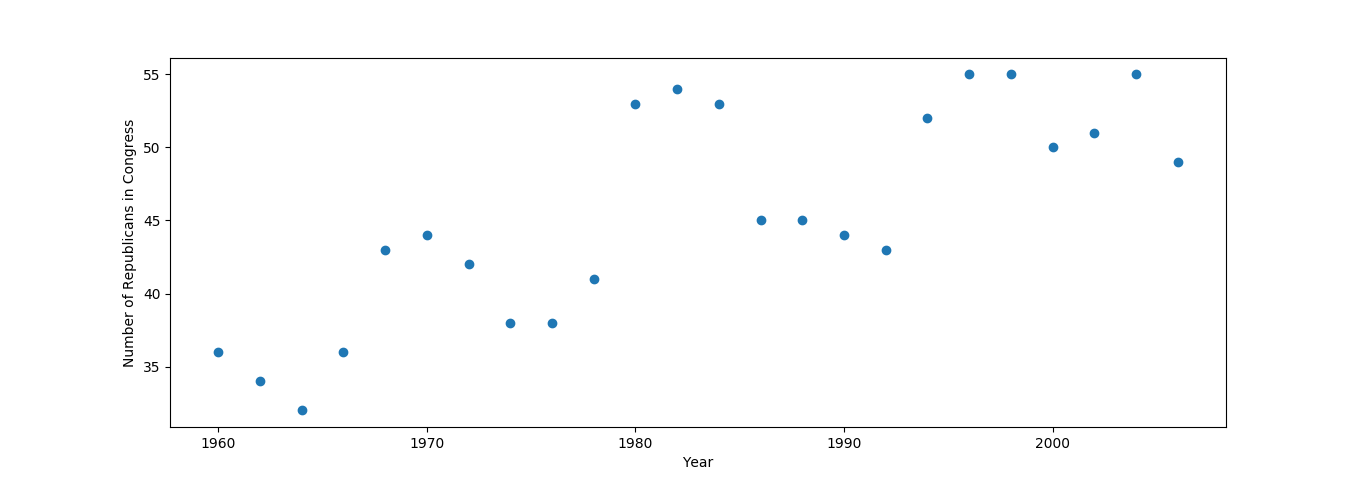
\includegraphics[width=\textwidth]{data/year-republicans}
\caption{Number of Republicans in the Senate.  The horizontal axis is the year, and the vertical axis is the number of Republicans.}
\label{fig:congress}
\end{figure}

\begin{figure}[h]
\centering
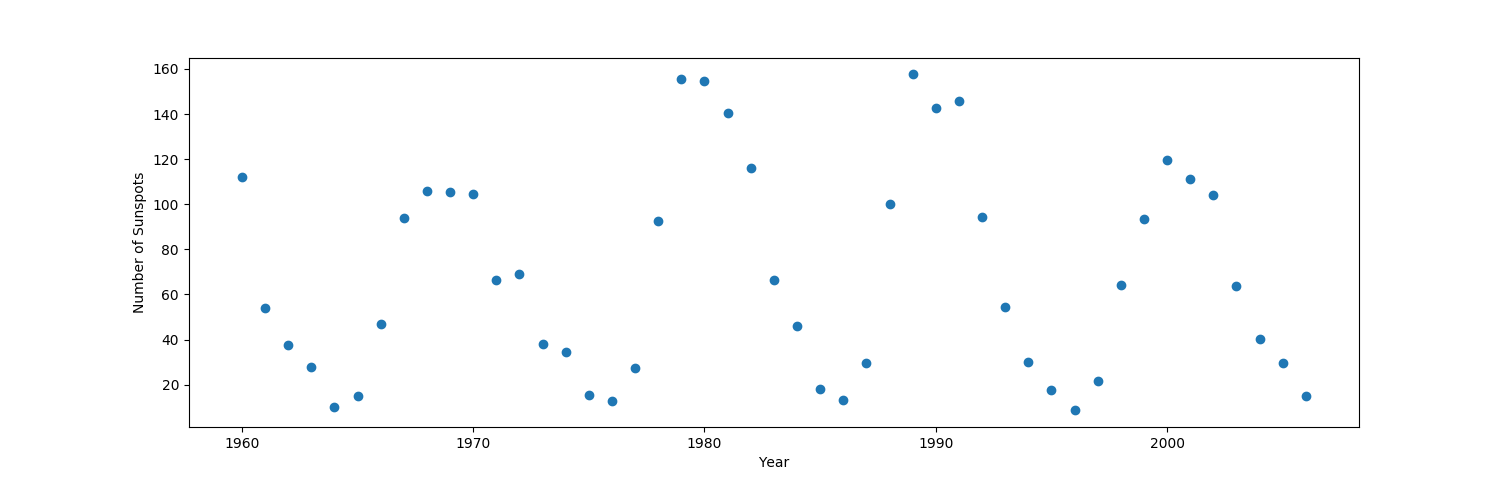
\includegraphics[width=\textwidth]{data/year-sunspots}
\caption{Number of sunspots by year.  The horizontal axis is the year, and the vertical axis is the number of sunspots.}
\label{fig:sunspots}
\end{figure}

Data Source: \url{http://www.realclimate.org/data/senators_sunspots.txt}

\begin{problem}[Modeling Changes in Republicans and Sunspots, 15pts] 

Implement basis function regression with ordinary least squares for
years vs. number of Republicans in the Senate. Some sample Python code
is provided in \verb|linreg.py|, which implements linear regression.
Plot the data and regression lines for the simple linear case, and for
each of the following sets of basis functions (only use (b) for years, skip for sunspots):
\begin{itemize}
	\item[(a)] $\phi_j(x) = x^j$ for $j=1, \ldots, 5$ 
    \item[(b)] $\phi_j(x) = \exp{\frac{-(x-\mu_j)^2}{25}}$ for $\mu_j=1960, 1965, 1970, 1975, \ldots 2010$
	\item[(c)] $\phi_j(x) = \cos(x / j)$ for $j=1, \ldots, 5$
	\item[(d)] $\phi_j(x) = \cos(x / j)$ for $j=1, \ldots, 25$
\end{itemize}
In addition to the plots, provide one or two sentences for each with
numerical support, explaining whether you think it is fitting well,
overfitting or underfitting.  If it does not fit well, provide a
sentence explaining why. A good fit should capture the most important
trends in the data.\\ 

\noindent Next, do the same for the number of sunspots vs. number of
Republicans, using data only from before 1985.  What bases provide the
best fit?  Given the quality of the fit, would you believe that the
number of sunspots controls the number of Republicans in the senate?

\end{problem}



\subsubsection*{Solution}


%%%%%%%%%%%%%%%%%%%%%%%%%%%%%%%%%%%%%%%%%%%%%
% Problem 3
%%%%%%%%%%%%%%%%%%%%%%%%%%%%%%%%%%%%%%%%%%%%%
\newpage
\begin{problem}[BIC, 15pts]

Adapted from $Biophysics: Searching\ for\ Principles$ by William Bialek.\\

\noindent Consider data $\mathcal{D} = \{(x_i, y_i)\}$ where we know that

    $$y_i = f(x_i ; \bold{a}) + \epsilon_i$$

\noindent where $f(x_i ; \bold{a})$ is a function with parameters $\bold{a}$, and $\epsilon_i \sim \mathcal{N}(0,\sigma^2)$ is an additive noise term.
We assume that $f$ is a polynomial with coefficients $\mathbf{a}$.
Consider the class of all polynomials of degree $K$. Each of these polynomials can be viewed as a generative model of our data, and we seek
to choose a model that both explains our current data and is able to generalize to new data. This problem explores the use of the Bayesian Information Criterion (BIC)
for model selection. Define the $\chi^2$ (\textit{chi-squared}) error term for each model of the class as:

$$\chi^2 =  \frac{1}{\sigma^2} \sum_{i=1}^N \left( y_i - \sum_{j=0}^K a_j x_i^j \right)^2 $$

\noindent Using this notation, a formulation of the BIC can be written as: 

$$-\ln P({x_i,y_i} | \text{model class} ) \approx \frac{N}{2} \ln (2\pi \sigma^2) - \sum_{i=1}^N \ln p(x_i) + \frac{1}{2} \chi^2_{min} + \frac{K}{2} \ln N $$ \\

\noindent where $\chi^2_{min}(K)$ denote the minimum value of the $\chi^2$ over the set of polynomial models with $K$ parameters. 
Finally, assume that $x_i \sim Unif(-5,5)$ and that each $a_j \sim Unif(-1,1)$. Let $K_{true} = 10$.

    \begin{itemize}
    
        \item[(a)] Write code that generates $N$ data points in the following way:
            \begin{enumerate}
                \item Generate a polynomial $f(x) = \sum_{j = 0}^{K_{true}} a_j x^j$ 
                \item Sample $N$ points $x_i$
                \item Compute $y_i = f(x_i) + \epsilon_i$ where $\epsilon$ is sampled from $\mathcal{N}(0, \sigma^2 = \frac{ \max_i f(x_i) - \min_i f(x_i) }{10})$.
            \end{enumerate}
        
        \item[(b)] For a set of $y_i$ generated above and a given $K$, write a function that minimizes $\chi^2$ for a polynomial of degree $K$ by solving for $\mathbf{a}$ using
                   numpy \texttt{polyfit}.                   Check for $N=20$ that $\chi^2_{min}(K)$ is a decreasing function of $K$. 
        
        \item[(c)] For $N=20$ samples, run $500$ trials. This involves generating a new polynomial for each trial, then from that polynomial, 20 sample data points $\{(x_i,y_i)\}$. For each trial, 
                          we can calculate the optimal $K$ by minimizing BIC. Compute the mean and variance of the optimal $K$ over 500 trials.
        
        \item[(d)] For $N$ ranging from $3$ to $3 \cdot 10^4$ on a log scale (you can use the function $3*np.logspace(0,4, 40)$ as your values of $N$), 
                   compute the mean and variance of the optimal $K$ over 500 trials for each $N$. Plot your results, where the x-axis is the number of samples ($N$) on a log-scale, 
                   and the y-axis is the mean value of the optimal $K$ with error bars indicating the variance over 500 trials. Verify that minimizing the BIC controls the complexity of the fit, 
                   selecting a nontrivial optimal $K$. You should observe that the optimal K is smaller than $K_{true}$ for small data sets, and approaches $K_{true}$ as you 
                   analyze larger data sets.
        
    \end{itemize}


\end{problem}

\subsubsection*{Solution}




%%%%%%%%%%%%%%%%%%%%%%%%%%%%%%%%%%%%%%%%%%%%%
% Problem 4
%%%%%%%%%%%%%%%%%%%%%%%%%%%%%%%%%%%%%%%%%%%%%
\newpage
\begin{problem}[Calibration, 1pt]
Approximately how long did this homework take you to complete?
\end{problem}
\textbf{Answer:}

\end{document}
